\chapter{System architecture}
% arquitectura del sistema
%API python
% web
\label{chap:architecture}

\textit{In this chapter the system architecture will be shown. We will explain how we have implemented the web server, the user interface and the automations created for it.}

\clearpage

\section{General Architecture}

%This chapter will serve as a description of the methodology that has been followed in order to develop the system and meet the requirements set out in the Chapter~\ref{chap:introduction}. As mentioned, this work arises from the need of tackling a problem in today's society, namely Eating Disorders. More specifically, the aim is to help in the early detection of such illnesses so that they can be treated as soon as possible.

The aim of this project is to help in the early detection of Eating Disorders so that they can be treated as soon as possible. To achieve that, the system's presentation should be easy to handle and understandable for the people who use it. Furthermore, it has to be visually appealing in order to motivate people with a potential Eating Disorder to use it. We want to include the option of performing some actions after the prediction is taken as well.

The system architecture that has been developed for this Master Thesis can be seen in the Figure~\ref{fig:architecture}, where you can find the interactions between the subcomponents in a simplified diagram.

% Mostrar esquema arquitectura
\begin{figure}[h]
    \centering
    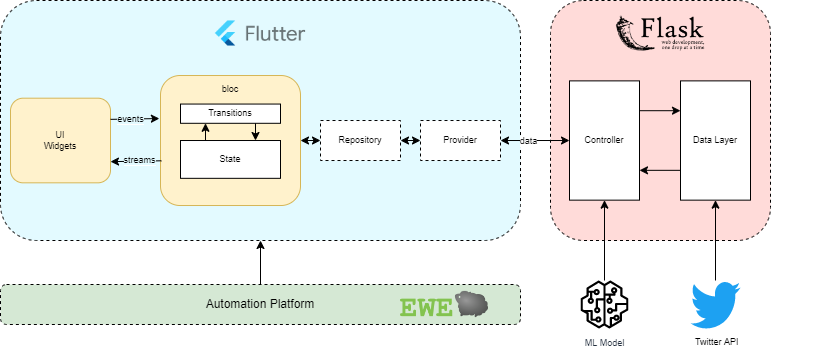
\includegraphics[width=1.05\textwidth]{img/architecture/architecture.png}
    \caption{Simplified diagram of the architecture of the system}
    \label{fig:architecture}
\end{figure}


In this figure you can see a simplified abstract diagram of the structure of our system, consisting of two distinct main elements, which are the server made with Flask and the user interface for which Flutter has been used. In the following we will break down this architecture and zoom in on the different parts to explain what the elements represented in the diagram above consist of and what function they have.

The presentation layer of this Master Thesis has been designed using a specific methodology based on states called bloc, which will be explained in this chapter. There are diferent parts that are part of this bloc architecture that need to be implemented in order to perform different actions that will enhance the user experience.

To serve this presentation layer with data, a server has been implemented in which an API has been constructed. The objective of this is to consult the information about the required user and predict the suffering of an Eating Disorder. This server makes calls to the Twitter API also to make the prediction using the Machine Learning model previously preloaded on the same server. The model that has been followed for implementing this part of the system is called Front Controller, which will be explained here.

Besides, we have integrated the system with an Automation Platform powered by EWE. It includes semantic automation to our system for helping us to include different actions that users can take after the prediction is performed. This enhances the features of the platform and as a consequence, the user experience. We will talk about this topic in a separated Section in this Chapter.

\section{Flask server}
\label{sec:server}
% Funciones que realiza: Extraccion datos, procesamiento y predicción
 In this section we are going to focus on the part that obtains and processes the data from our application in order to be able to make a prediction about the user we want to analyse. The basic functions of this are data extraction, data processing and the generation of a prediction that is returned in JSON format as a response, along with additional information.
 
 We needed a technology that was fast and light as we didn't want to overcomplicate the text processing, we just wanted it to be easy to query to get the best user experience and reduce waiting times. For this reason we chose Flask, a fairly mature lightweight framework for Python, which allows us to set up a server in a matter of seconds and process requests quickly.
 
 
 
 % MODELO SEGUIDO en  arquitectura: FRONT CONTROLLER
 The architecture pattern followed to implement this Flask server is the Front Controller model, which can be seen in the Figure~\ref{fig:front-controller}. This model is based on a controller that handles all requests from a server, which is useful to achieve flexibility and reuse code without redundancy.

 
\begin{figure}[h]
    \centering
    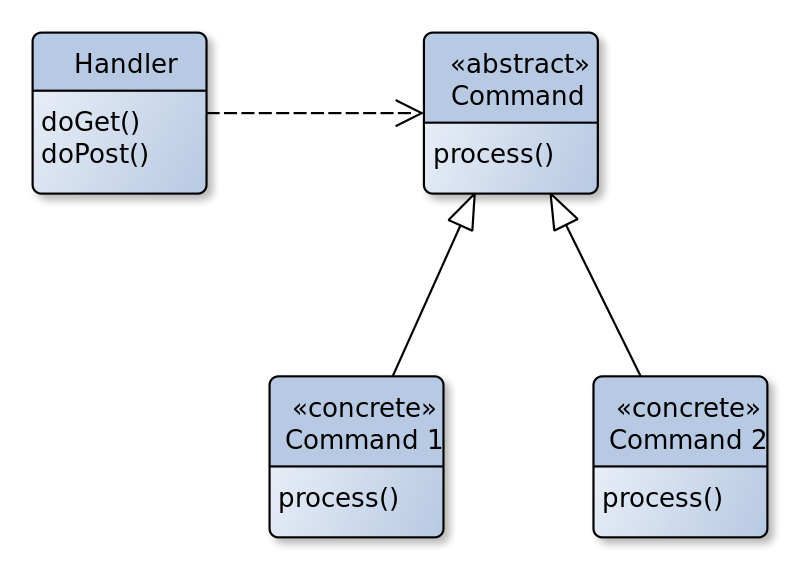
\includegraphics[width=0.65\textwidth]{img/architecture/Front_Controller.png}
    \caption{Example of Front Controller architecture}
    \label{fig:front-controller}
\end{figure}

These front controllers are normally used in web applications like the one in this project to implement flows. It serves to simplify navigation between screens and is invoked every time calls are made to the server. This Front Controller handles all the tasks common to the application, such as session, caching and in our case routing and invocation of data extraction through implemented methods.

This was the most interesting option and the one that best suited what we were looking for in this Master Thesis, as we took into account the features that we needed and the simplicity the model provides to perform and implement those features. 

The features that we required from this sever are as mentioned before, three main tasks, which are data extraction, data processing with its prediction, and data serving through the API which we will break them out in the following.

% 1. Extraccion de datos
\myparagraph{Data extraction}
The focus of this project is on the social network Twitter and because of this, we need to extract information from Twitter in order to achieve our goal. We want to analyse per user the suffering of an Eating Disorder so we need to extract the latest tweets of a specific person in order to treat them and introduce them as input to our model.

For this, we used a Python-based tool called snscrape~\cite{JustAnot83:online}, which can extract data from the Twitter API without us having to authenticate ourselves. 

This snscrape Python package that can be easily installed using the pip manager. It allows us to take as many tweets as we want from a profile, and put them in a text file in JSON format. An example of this can be seen in the code block described in Appendix~\ref{appendix:JSONsnscrape}.

So, it was decided to use snscrape for its simplicity and for not needing to authenticate to the API. With the command written in the Code~\ref{code:snscrape} we can access the 1000 most recent tweets of the user with the identifier \$username and save them in JSON format in the file user-tweets.json.

Subsequently, we will read this file to be able to process the information taken. The tool has more functionalities such as searching Twitter (twitter-search) or consulting a profile (twitter-profile) but this one is enough for the given approach.

\begin{lstlisting}[caption={Command executed for obtaining tweets}, label={code:snscrape}]
snscrape --jsonl --max-results 1000 twitter-user $username > user-tweets.json
\end{lstlisting}

Once we have the file ready, we read it using the pandas library in order to ingest it into our model, preprocessing it beforehand. This file is given a temporal character because after reading the file, it is deleted from the server so as not to generate overload. Now, in the next paragraph, we will explain how we preprocess the text once it is read.

% 2. Procesamiento de datos (empaquetamiento de modelo) / wordcloud y prediccion
\myparagraph{Data processing and prediction}
We need to process the data obtained from twitter in our platform, so we will treat the information in a similar way in this Flask server to the one explained in~\ref{sec:preprocessing}, as we want our model to work in a similar way as it did with the validation data because it gave us good results. 


So, what we do is reuse the code written in Code~\ref{code:preprocessing} for this data extracted from Twitter. As a result we get an array of words from the last tweets published by the user in question.

%Wordcloud
In addition, we took the opportunity of having this to create more statistics and to give the user more insights. For example, we have implemented the creation of a wordcloud that reflects the most used words and their frequency in a very intuitive graphical way.

% 3. Como se sirven los datos: rutas y por JSON --> API
\myparagraph{Data serving through API}
%JSON Format and wordcloud img processing
To serve the prediction and additional statistics the API has been programmed as above. This API has a dedicated path to return the extracted results in JSON format.

The simplified output obtained by querying the API as can be seen in the Code~\ref{code:jsonapi} is a composition of the prediction result, user information and the wordcloud image in base64 format. This information is then used in the Flutter part to build the user interface.

%% METER EJEMPLO JSON
\begin{lstlisting}[caption={JSON output from API}, label={code:jsonapi}]
{
    "prediction": "0", 
    "username": "elonmusk", 
    "pic": "https://pbs.twimg.com/profile_images/1529956155937759233/Nyn1HZWF.jpg", 
    "wordcloud": "iVBORw0KGgoAAAANSUhEUgAAAZAAAADICAIAAAB..."
}
\end{lstlisting}


In order to be able to send the wordcloud image through the API, it has to be encoded in base64 format. Subsequently, it has to be decoded in the application part in order to be displayed.\\

Besides these mentioned tasks that are directly related to the web server functioning, we have also equipped the module with a Semantic Events Trigger. This block is throwing an event against the Task Automation Server in order to trigger actions that are reflected on the user interface. We will talk about this integration in the Section~\ref{sec:taskautomation}.

In the following section we will focus on the application that the user uses, presenting its parts, the model used in its design and its structure.
\section{Flutter application}
% Presentacion de la aplicacion
The application aims to have a clear and guided user experience that engages the user for using it. It should have a clear flow for easing its manipulation and really help the person who uses it. Because of that we used Flutter for implementing it.

%Multiplataforma
It is a Flutter-based as it is mentioned, so that implies that it is a cross-platform application that can be run in Android, iOS and web, which make it polivalent. Its content is dinamically treated so it adjusts to all kinds and sizes of screen, which has been also take into account in the design process.

% Diseño de la app: BLOC
The design pattern followed is called BloC, which makes our application based on separate components. These components contain only the business logic, \textit{i.e.} the logic that determines how information can be created, stored and changed.

BLoC is widely used in applications developed in Flutter, as it is based on widgets and this pattern provides the support to communicate these widgets with other components of the application.

This communication is done through the issuing of events from the UI as shown in the Figure~\ref{fig:bloc}. BLoC components receive this events and take the actions that are needed, changing their state. Afterwards, they emit back stream back to the UI to make the relevant changes to the interface. 

\begin{figure}[h]
    \centering
    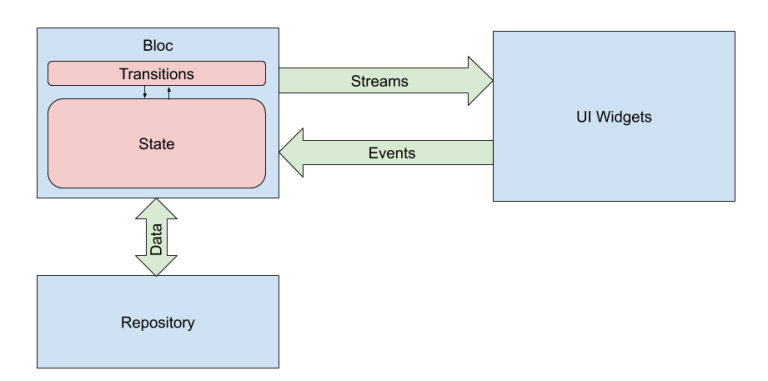
\includegraphics[width=0.85\textwidth]{img/architecture/bloc.png}
    \caption{BLoC architecture}
    \label{fig:bloc}
\end{figure}

In turn, our BLoC-based application is packed with repositories, which serve to obtain data necessary for the application, as in this case is the prediction of our system issued by the Flask server explained before. The repository of our system provides access to long-term state data, in our case via API.

Furthermore, we have connected this user interface with the Task Automation Server. When a positive prediction is done, the webserver will trigger an event against the automation platform and the response of this platform will be received in our Flutter application. With this data some actions are displayed in user screen in order to help to advance in the diagnosis process.

\section{Task Automation}
\label{sec:taskautomation}
As mentioned before, we have integrated semantic task automation in our system in order to enhance the functionalities of our platform and also the user experience. We have used a Task Automation Service (TAS) hosted by GSI department of the Universidad Politécnica de Madrid which provide us with the ability of online automation.

Our system will be based on Evented WEb (EWE) as we have indicated in the Chapter~\ref{chap:state-of-art}. This ontology has four major classes on its core which are Channel, Event, Action and Rule, and we need to have a semantic representation for putting an automation in place. In this Section we will detail the representations developed for this Master Thesis

Before that, for setting the ground, we would like to pose the architecture on which this semantic task automation is constructed. As discussed it is a service which is running online which is constructed as the Figure~\ref{fig:ewearchitecure} is shown.

\begin{figure}[h]
    \centering
    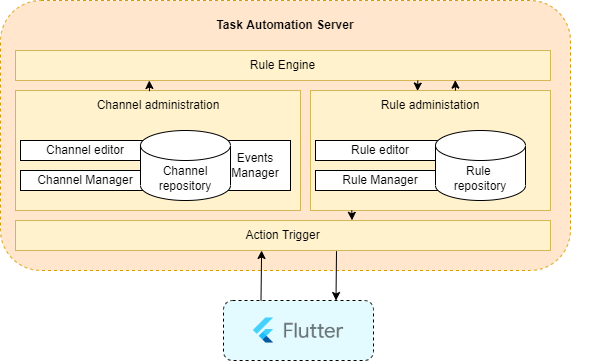
\includegraphics[width=0.85\textwidth]{img/architecture/EWEarchitecture.png}
    \caption{EWE architecture for our system}
    \label{fig:ewearchitecure}
\end{figure}

As it can be seen this Automation Server is connected both to our user interface and our web server. When a positive prediction is performed in the Flask server, an event is triggered, arriving to the Events Manager of the Task Automation Server. Once the event is received, it interacts with the Rule Engine which decides what to do with that event depending on the configured rules.

The engine is the one in charge of running the rules, which are patterns that are defined in the EWE ontology that create relations among objects. In the rules, relationships between different channels, events and actions are defined.

Besides, Rule Engine is connected with the Channel and the Rule Administrators, which provide the necessary resources for dispatching the rule. These are modules that have the same purpose but for different objects supported by the ontology. Both have a repository where the objects are stored and also they are provided with a manager and an editor, which serve for modifying the objects or even delete them.

When the rule is processed in the Rule Engine, it is contacting the Actions Trigger which activates the action that is indicated. This Actions Trigger is connected directly to the Flutter Interface, unleashing the necessary process that are desired for the user.

% ARCHITECTURE: pillar de aqui https://books.google.es/books?hl=es&lr=&id=HhKhDQAAQBAJ&oi=fnd&pg=PA33&ots=1Q4idJtH39&sig=6-uS1BX6NGtWcwug1GOMoIlns1s&redir_esc=y#v=onepage&q&f=false

We had to define a semantic model of our system in order to automatise the actions we want to take. These actions recommend the user to talk to friends, contact an organisation or make an appointment with a specialized doctor. These actions are triggered when a positive response is made.


% Meter representacion creada
This created and custom representation with the declaration of channel, events and actions can be seen in the following Code~\ref{code:ewerepresentation}.

\begin{lstlisting}[label={code:ewerepresentation}, caption={Custom semantic representation implemented}]
###################################
# Channel definition
###################################
ewe-ed:EDPrediction a owl:Class ;    
    rdfs:label "Prediction of Eating Disorder made by platform"@en ;
    rdfs:comment "This channel represents the prediction emited by the system"@en
    rdfs:subClassOf ewe:Channel .

###################################
# Events definition
###################################

ewe-ed:EDPredictionPositive a owl:Class ;
    rdfs:label "User has been predicted as positive in Eating Disorder"@en ;
    rdfs:comment "This Trigger fires when a prediction is positive in Eating Disorder."@en ;
    rdfs:subclassOf ewe:Event ;
    rdfs:domain ewe-ed:EDPrediction .

ewe-ed:EDPredictionNegative a owl:Class ;
    rdfs:label "User has been predicted as negative in Eating Disorder"@en ;
    rdfs:comment "This Trigger fires when a prediction is negative in Eating Disorder."@en ;
    rdfs:subclassOf ewe:Event ;
    rdfs:domain ewe-ed:EDPrediction .

###################################
# Actions definition
###################################
ewe-ed:RecommendFriends a owl:Class ;
    rdfs:label "Recommend Friends"@en ;
    rdfs:comment "This action will tell to call a friend."@en ;
    rdfs:subclassOf ewe:Action ;
    rdfs:domain ewe-ed:EDPrediction .

ewe-ed:RecommendNGO a owl:Class ;
    rdfs:label "Recommend NGO"@en ;
    rdfs:comment "This action will tell to contact an organisation"@en ;
    rdfs:subclassOf ewe:Action ;
    rdfs:domain ewe-ed:EDPrediction .

ewe-ed:RecommendDoctor a owl:Class ;
    rdfs:label "Recommend Doctor"@en ;
    rdfs:comment "This action will tell to contact an expert"@en ;
    rdfs:subclassOf ewe:Action ;
    rdfs:domain ewe-ed:EDPrediction .

\end{lstlisting}

Besides this, we have added a set of rules which trigger the actions that we have implemented there when a prediction is positive. All of this will be charged into the Task Automation Server so it can understand and talk our system's language.

